
\documentclass{IEEEtran}
\usepackage[spanish]{babel}
\usepackage[utf8]{inputenc}
\usepackage{enumerate}
\usepackage{cite}
\usepackage{graphicx}  
\usepackage{subfig}
\usepackage{float}
\usepackage{tikz}
\usepackage{pgfplots}
\usetikzlibrary{pgfplots.dateplot}
\usepackage{pgfplotstable}
\usepackage{filecontents}

% correct bad hyphenation here
\hyphenation{op-tical net-works semi-conduc-tor}


\begin{document}
%
% paper title
% can use linebreaks \\ within to get better formatting as desired
% Do not put math or special symbols in the title.
\title{Práctica 3: Difuminado de imagen CUDA}


% author names and affiliations
% use a multiple column layout for up to three different
% affiliations
\author{\IEEEauthorblockN{Andrés Fernando Román Arévalo, Ronald Sarmiento\\}
\IEEEauthorblockA{Email:afromana@unal.edu.co, roasarmientoga@unal.edu.co\\}
\IEEEauthorblockA{Universidad Nacional Bogotá, Colombia \\}
}


% make the title area
\maketitle

\begin{figure}[!t]
\centering

\includegraphics[width=2.5in]{logo_unal}
\label{fig_sim}
\end{figure}
% As a general rule, do not put math, special symbols or citations
% in the abstract
\begin{abstract}
El siguiente informe presenta como se llevo a cabo la paralelización mediante el uso de la plataforma de programación en paralelo CUDA   del efecto borroso y los resultados que se obtuvieron tanto de Speed Up como de Time Response para los distintas resoluciones  de imagenes (720p, 1080p y 4k)) y de kernels (2,3,4,5, 6,7, 8,9, 10,11 ,12 13 y 14) asi como la comparación con los tiempos obtenidos en CPU
\end{abstract}

% no keywords


\IEEEpeerreviewmaketitle



\section{Introducción.}
% no \IEEEPARstart
Una de las tareas altamente demandada en la actualidad es el procesamiento de imagenes cada vez de una mayor resolución para lo cual se requiere un alto nivel de computo. A partir de esto han surgido innumerables algoritmos que permiten paralelizar las distintas operaciones de procesamiento de imagenes como lo es la del efecto difuminado.\\\\
% You must have at least 2 lines in the paragraph with the drop letter
% (should never be an issue)
Aun asi paralelizar tiene su limite que es explicado en la Ley de Amdahl, la cual establece que hay un punto en que paralelizar ya no ofrece mejoras significativas de rendimiento e incluso por el contrario puede llevar al deterioro del mismo.\\\\

Al momento de hacer procesamiento de imagenes se utiliza distintas operaciones matriciales.En el caso del efecto borroso se realiza una convolucion entre la matriz que representa la imagen y el kernel

\begin{figure}[H]
  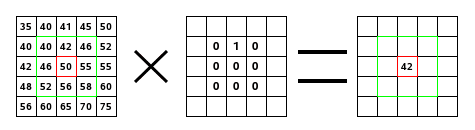
\includegraphics[width=\linewidth]{matriz.png}
  \caption{Convolucion matricial}
  \label{fig:boat1}
\end{figure}
\subsection{Creación del efecto difuminado}

Mas especificamente se utilizo la tecnica de difuminado conocida como Blur el cual consiste en intercambiar cada pixel de la imagen por un promedio de los valores RGB que se encuentras en los pixeles adyacentes a el. El nivel de difuminado esta determinado por el kernel y el tamaño da el rango que se toma para evaluar el promedio. Es decir, si se escoge un kernel de 5 significa que cada pixel sera cambiado por el promedio que hay en los promedios de la matriz 5x5 cuyo centro es el pixel en cuestion.

\section{Algoritmo de paralización.}
La paralelizacion se realizo mediante asignación tipo blockwise es decir que se tomo la imagen y se dividio a lo alto en filas y cada una de estas se asigno a un hilo. Es decir que un caso hipotetico donde se quiera aplicar el efecto difuminado a una imagen con un alto de 368 pixeles,se  lanzan 4 hilos donde el hilo 1 se le asignaba la fila 1(del pixel 0 al 92), al 2 la fila 2(del pixel 92 al 184 ), al 3 la columna 3(del pixel 184 al 276)  y al 4 la  columna 4(del pixel 276 al 368) . Para mayor clarificación detras de la idea que se uso para la paralización, la siguiente imagen:

\begin{figure}[H]
  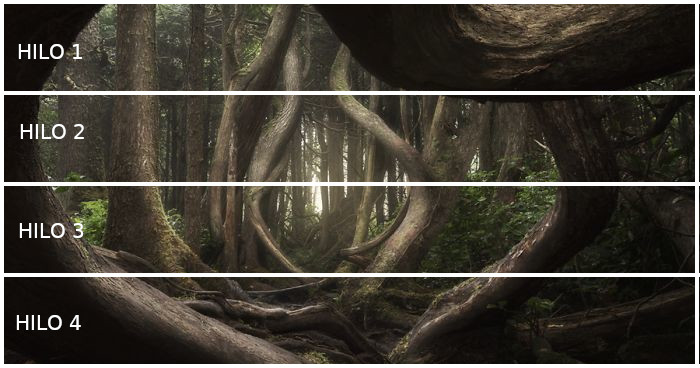
\includegraphics[width=\linewidth]{mod.jpg}
  \caption{Algoritmo de paralelización}
  \label{fig:boat2}
\end{figure}

El ejemplo anterior muestra el caso en el cual se lanza un solo bloque con 4 hilos. Pero para el experimento se decidio lanzar la máxima cantidad de hilos posibles es decir el alto de la imagen para calcular tanto el time response como el speed up en base al tamaño del kernel
\section{Experimentos y resultados.}
Antes de mostrar los resultados obtenidos y compararlos con los que se obtuvieron al paralelizar el efecto difuso que se obtuvo con CUDA en comparación con los de CPU(POSIX Y OpenMP), es necesario decir que se corrio en el entorno de Google Colab. 


\subsection{Resultados}
Como primera medida se utilizo el time response o tiempo de ejecución de un programa, donde para cada imagen se crearon sus corresponientes gráficas donde en eje horizontal se colocaron el tamaño del kernel que ejecutaba el programa y en el eje vertical el tiempo que tardo.\\
A continuacion se presentan las gráficas correspondientes:\\
\begin{itemize}
    \item \textbf{Imagen de 720p}
    
    \begin{tikzpicture}
\begin{axis}[
xticklabels={},
extra x ticks={1,2,3,4,5,6,7,8,9,10,11,12,13,14},
title={Time Response 720p},
xlabel={Tamaño del kernel},
ylabel={Tiempo},
nodes near coords, 
 every node near coord/.append style={font=\tiny,yshift=-1.6pt},
 nodes near coords style={/pgf/number format/.cd,precision=3},
]
\addplot coordinates { (2,0.375) (3,0.355) (4,0.420) (4,0.383) (6,0.469) (7,0.396) (8,0.419) (9,0.417) (10,0.494) (11,0.492) (12,0.563) (13,0.560) (14,0.691)};
\end{axis}
\end{tikzpicture}



\item \textbf{Imagen de 1080p}

    \begin{tikzpicture}
\begin{axis}[
xticklabels={},
extra x ticks={1,2,3,4,5,6,7,8,9,10,11,12,13,14},
title={Time Response 1080p},
xlabel={Tamaño del kernel},
ylabel={Tiempo},
nodes near coords, 
 every node near coord/.append style={font=\tiny,yshift=-1.6pt},
 nodes near coords style={/pgf/number format/.cd,precision=3},
]
\addplot coordinates { (2,0.377) (3,0.372) (4,0.441) (4,0.433) (6,0.530) (7,0.526) (8,0.629) (9,0.633) (10,0.848) (11,0.845) (12,1.121) (13,1.128) (14,1.452)};
\end{axis}
\end{tikzpicture}

\item \textbf{Imagen de 4k}

    \begin{tikzpicture}
\begin{axis}[
xticklabels={},
extra x ticks={1,2,3,4,5,6,7,8,9,10,11,12,13,14},
title={Time Response 4k},
xlabel={Tamaño del kernel},
ylabel={Tiempo},
nodes near coords, 
 every node near coord/.append style={font=\tiny,yshift=-1.6pt},
 nodes near coords style={/pgf/number format/.cd,precision=3},
]
\addplot coordinates { (2,1.391) (3,1.397) (4,1.717) (5,1.734) (6,2.240) (7,2.237) (8,2.9) (9,2.898) (10,3.833) (11,3.830) (12,4.755) (13,4.768) (14,6.078)};
\end{axis}
\end{tikzpicture}


\end{itemize}

Como se puede observar en las gráficas anteriores el time response del código tiene cierta tendencia de  empeorar  conforme se aumenta el tamaño del kernel, como es el comportamiento esperado.\\

Otra medida que se considero determinar para medir el rendimiento de los hilos en el programa es el speed up que para este caso se calculo como la división entre el mejor tiempo en CPU contra con los mejores tiempos en GPU \\
A continuación se presentan las gráficas correspondientes:

\begin{figure}[H]
  
\includegraphics[width=\linewidth]{memev.jpg}
  \caption{Speed Up}
  \label{fig:boat2}
\end{figure}

\section*{Conclusiones.}
\begin{itemize}
  \item Entre mas grande es el kernel con el que se trabaja se demora un tiempo superior en realizar el efecto difuminado debido a que realiza mas operaciones al momento de calcular el promedio del kernel, haciendo que el costo computacional sea superior
\end{itemize}


\noindent 


\begin{thebibliography}{00}
\bibitem{b2} Pedraza, C. (2019). Diapositivas de clase.
\bibitem{b1}David, K. and Wen-Mei, H. (2010). Programming massively parallel processos. 2nd ed. Morgan Kaufmann.
\bibitem{b2} Thomas, R. and Gudula, R. (2010). Parallel Programming. 1st ed. Springer.
\bibitem{b2} En.wikipedia.org. $(2019). Box blur.  Available at: https://en.wikipedia.org/wiki/Box_blur.$
\end{thebibliography}




% that's all folks
\end{document}


